\chapter{Desarrollo del Trabajo}
En esta sección se desarrolla el tratamiento formal del oscilador armónico, partiendo de su formulación clásica como sistema dinámico fundamental y avanzando hacia su descripción cuántica. En primer lugar, se presenta el oscilador armónico clásico como base conceptual para la cuantización. Posteriormente, se construye el Hamiltoniano cuántico y se obtiene el espectro energético mediante el método algebraico basado en operadores de creación y aniquilación. A continuación, se analizan las autofunciones del sistema y se establece la equivalencia formal con el método analítico derivado de la ecuación de Schrödinger. Finalmente, se discuten algunas aplicaciones físicas relevantes que evidencian la importancia del modelo en distintos ámbitos de la física moderna.

\section{El oscilador armónico clásico}
El oscilador armónico clásico constituye el modelo paradigmático del movimiento periódico en física. Describe el comportamiento de una partícula sometida a una fuerza restauradora proporcional y opuesta a su desplazamiento respecto de una posición de equilibrio estable. Este sistema no solo aparece en el estudio de masas unidas a resortes ideales, sino que representa una aproximación universal para describir sistemas físicos en las proximidades de un mínimo de energía potencial.

La importancia del oscilador armónico radica en su carácter general: cualquier sistema cuya energía potencial posea un mínimo estable puede aproximarse localmente mediante una función cuadrática. Esta propiedad explica su presencia en múltiples áreas de la física, desde la mecánica clásica hasta la teoría cuántica de campos. En particular, el formalismo matemático desarrollado para el oscilador armónico clásico servirá como punto de partida para su formulación cuántica, donde las variables dinámicas serán promovidas a operadores y la energía adquirirá una estructura discreta.

\subsection{Descripción física y potencial armónico}
En su forma más simple, el sistema puede representarse como una partícula de masa $m$ unida a un resorte ideal de constante elástica $k$. La dinámica está gobernada por la ley de Hooke,

\[
F = -kx,
\]

donde $x$ es el desplazamiento respecto del equilibrio. Aplicando la segunda ley de Newton se obtiene

\[
m\ddot{x} + kx = 0.
\]

Definiendo la frecuencia angular natural del sistema como

\[
\omega = \sqrt{\frac{k}{m}},
\]

la ecuación de movimiento adopta la forma

\[
\ddot{x} + \omega^2 x = 0,
\]

cuya solución describe un movimiento periódico.

Desde el punto de vista energético, la fuerza restauradora deriva de un potencial cuadrático

\[
V(x) = \frac{1}{2} k x^2 = \frac{1}{2} m\omega^2 x^2,
\]

cuya forma parabólica caracteriza al oscilador armónico. Más generalmente, cualquier potencial físico $V(x)$ con un mínimo estable puede aproximarse, para pequeñas oscilaciones, por una expresión cuadrática alrededor del punto de equilibrio. Esta propiedad explica el carácter universal del oscilador armónico como modelo físico.

La energía total del sistema se expresa mediante el Hamiltoniano clásico,

\[
H(x,p) = \frac{p^2}{2m} + \frac{1}{2} m\omega^2 x^2,
\]

donde $p = m\dot{x}$ es el momento lineal. Esta expresión será el punto de partida para la formulación cuántica del problema, en la que las variables dinámicas se promoverán a operadores y la energía adquirirá una estructura discreta.
\subsection{Hamiltoniano clásico del oscilador}

El oscilador armónico clásico puede describirse de manera natural dentro del formalismo hamiltoniano. 
La energía total del sistema se compone de energía cinética y energía potencial,

\[
E = T + V = \frac{p^2}{2m} + \frac{1}{2}k x^2,
\]

donde $p = m\dot{x}$ es el momento lineal.

Introduciendo la frecuencia angular $\omega = \sqrt{k/m}$, el Hamiltoniano del sistema adopta la forma

\[
H(x,p) = \frac{p^2}{2m} + \frac{1}{2}m\omega^2 x^2.
\]

Este Hamiltoniano representa la función energía del sistema y genera la dinámica a través de las ecuaciones canónicas de Hamilton,

\[
\dot{x} = \frac{\partial H}{\partial p}, 
\qquad
\dot{p} = -\frac{\partial H}{\partial x}.
\]

De estas ecuaciones se recupera directamente la ecuación diferencial del movimiento armónico,

\[
\ddot{x} + \omega^2 x = 0.
\]

La formulación hamiltoniana resulta especialmente importante, pues será el punto de partida para la transición al tratamiento cuántico.

\subsection{Solución clásica y significado físico}

La ecuación de movimiento del oscilador armónico clásico,

\[
\ddot{x} + \omega^2 x = 0,
\]

es una ecuación diferencial lineal cuya solución general es

\[
x(t) = A \cos(\omega t) + B \sin(\omega t),
\]

donde $A$ y $B$ dependen de las condiciones iniciales. 
Equivalentemente,

\[
x(t) = C \cos(\omega t + \phi),
\]

siendo $C$ la amplitud y $\phi$ la fase inicial.

El movimiento es periódico, con período

\[
T = \frac{2\pi}{\omega},
\]

y frecuencia angular $\omega = \sqrt{k/m}$. 
La energía total del sistema permanece constante,

\[
E = \frac{p^2}{2m} + \frac{1}{2}m\omega^2 x^2,
\]

intercambiándose continuamente entre energía cinética y potencial.

Desde el punto de vista físico, el oscilador armónico describe pequeñas oscilaciones alrededor de una posición de equilibrio estable. 
Dado que cualquier potencial suave puede aproximarse por una función cuadrática en las cercanías de un mínimo, el oscilador armónico constituye una aproximación universal para sistemas físicos sometidos a pequeñas perturbaciones.

\section{Solución del oscilador armónico cuántico}
	
La transición del oscilador armónico clásico al tratamiento cuántico se realiza mediante la promoción de las variables dinámicas clásicas a operadores que actúan sobre un espacio de estados, de acuerdo con los postulados fundamentales de la mecánica cuántica formulados por Schrödinger \citep{schrodinger1926a} y la estructura algebraica introducida por Heisenberg \citep{heisenberg1925} y desarrollada sistemáticamente por Born y Jordan \citep{born1925, bornheisenberg1926}. 

En el marco cuántico, la posición $x$ y el momento $p$ dejan de ser magnitudes numéricas y pasan a representarse mediante operadores hermíticos que satisfacen la relación de conmutación canónica

\[
[\hat{x},\hat{p}] = i\hbar,
\]

la cual constituye el fundamento estructural de la teoría cuántica \citep{bornheisenberg1926}. Esta modificación altera profundamente la estructura matemática del problema y conduce, de manera natural, a un espectro energético discreto.

El oscilador armónico cuántico es, además, uno de los pocos sistemas que admiten solución analítica exacta. En lo que sigue se derivarán tanto el espectro de energía como las autofunciones completas mediante dos enfoques complementarios: el método algebraico introducido por Dirac \citep{dirac1930}, basado en operadores de creación y aniquilación, y el método analítico diferencial derivado de la ecuación de Schrödinger \citep{schrodinger1926b}. La equivalencia de ambos procedimientos constituye una validación explícita de la consistencia interna de la mecánica cuántica, demostrando que formalismos aparentemente distintos describen la misma estructura física subyacente.

	
\subsection{Planteamiento del problema}
	
Buscamos resolver la ecuación de Schrödinger independiente del tiempo \citep{schrodinger1926a}:
	
\begin{equation}
	\hat{H}\psi(x) = E\psi(x)
\end{equation}
	
donde el hamiltoniano para una partícula de masa $m$ en un potencial armónico de frecuencia angular $\omega$ es:
	
\begin{equation}
    \hat{H} = -\frac{\hbar^2}{2m}\frac{d^2}{dx^2} + \frac{1}{2}m\omega^2 x^2
\end{equation}
	
Esta forma del hamiltoniano combina el operador de energía cinética cuántico con el potencial armónico clásico 
\(
V(x) = \frac{1}{2}m\omega^2 x^2,
\)
correspondiente a una fuerza restauradora lineal \(F=-kx\), característica del oscilador armónico clásico.

	
Explícitamente, debemos resolver:

\begin{equation}
    -\frac{\hbar^2}{2m}\frac{d^2\psi}{dx^2} + \frac{1}{2}m\omega^2 x^2 \psi(x) = E\psi(x)
    \label{eq:schrodinger_oac}
\end{equation}

\textbf{Condiciones de frontera:} Para que $\psi(x)$ sea normalizable y represente un estado físico, requerimos:

\begin{equation}
    \lim_{x \to \pm\infty} \psi(x) = 0
\end{equation}

y

\begin{equation}
    \int_{-\infty}^{\infty} |\psi(x)|^2 dx = 1
\end{equation}

\textbf{Objetivo:} Encontrar:
\begin{enumerate}
    \item Los valores de energía $E_n$ permitidos (espectro)
    \item Las funciones de onda $\psi_n(x)$ correspondientes (autofunciones)
\end{enumerate}

Estos dos elementos constituyen la solución completa del problema cuántico.
	
	
\subsection{Solución algebraica mediante operadores}

El método algebraico, desarrollado por Dirac en "The Principles of Quantum Mechanics" (1930) \cite{dirac1930}, obtiene el espectro y estados del OAC sin resolver ecuaciones diferenciales, usando únicamente álgebra de operadores.

\subsubsection{Operadores de creación y aniquilación}

Definimos los operadores \cite{dirac1930}:

\begin{equation}
	\hat{a} = \sqrt{\frac{m\omega}{2\hbar}}\left(\hat{x} + \frac{i}{m\omega}\hat{p}\right)
\end{equation}

\begin{equation}
	\hat{a}^\dagger = \sqrt{\frac{m\omega}{2\hbar}}\left(\hat{x} - \frac{i}{m\omega}\hat{p}\right)
\end{equation}

Estos operadores no son hermitianos: $\hat{a}^\dagger \neq \hat{a}$.
De hecho, son adjuntos hermíticos entre sí: $(\hat{a})^\dagger = \hat{a}^\dagger$. Esto significa que \textbf{no representan observables físicos directamente}. Su utilidad es algebraica: actúan como operadores de ``escalera'' que permiten subir y bajar entre niveles de energía, sin ser ellos mismos cantidades medibles.

Sin embargo, combinaciones de $\hat{a}$ y $\hat{a}^\dagger$ pueden formar operadores hermitianos que sí son observables, como el operador número $\hat{N} = \hat{a}^\dagger\hat{a}$ o los operadores de posición y momento.\\

Podemos despejar estas relaciones para expresar $\hat{x}$ y $\hat{p}$ en términos de $\hat{a}$ y $\hat{a}^\dagger$:

\begin{align}
	\hat{x} &= \sqrt{\frac{\hbar}{2m\omega}}(\hat{a} + \hat{a}^\dagger) \\
	\hat{p} &= i\sqrt{\frac{m\omega\hbar}{2}}(\hat{a}^\dagger - \hat{a})
\end{align}

\subsubsection{Álgebra bosónica y relación de conmutación fundamental}

De la relación de conmutación canónica de  \cite{born1925} $[\hat{x}, \hat{p}] = i\hbar$, derivamos (ver Apéndice~\ref{sec:born1925}):

\begin{equation}
	[\hat{a}, \hat{a}^\dagger] = 1
	\label{eq:conmutador}
\end{equation}

Esta es la relación fundamental que gobierna todo el sistema y es la base del álgebra bosónica desarrollada en el trabajo fundamental de Born, Heisenberg y Jordan \citep{bornheisenberg1926}.

\subsubsection{Factorización del hamiltoniano}

Sustituyendo las expresiones de $\hat{x}$ y $\hat{p}$ en el hamiltoniano:

\begin{align}
	\hat{H} &= \frac{\hat{p}^2}{2m} + \frac{1}{2}m\omega^2\hat{x}^2 \\
	&= \hbar\omega\left(\hat{a}^\dagger\hat{a} + \frac{1}{2}\right)
\end{align}

Definiendo el \textbf{operador número} \cite{dirac1930}:

\begin{equation}
	\hat{N} = \hat{a}^\dagger\hat{a}
\end{equation}

el hamiltoniano se escribe:

\begin{equation}
	\boxed{\hat{H} = \hbar\omega\left(\hat{N} + \frac{1}{2}\right)}
	\label{eq:hamiltoniano_factorizado}
\end{equation}

Esta factorización constituye uno de los resultados más importantes del formalismo algebraico introducido por Dirac \citep{dirac1930}.


\subsubsection{Derivación algebraica del espectro}
Buscamos estados con número definido de cuantos. Estos son \textbf{autoestados} del operador número $\hat{N}$: estados que permanecen iguales (salvo un factor numérico) cuando $\hat{N}$ actúa sobre ellos.

Supongamos que existe un autoestado $|n\rangle$ del operador número con autovalor $n$:

\begin{equation}
	\hat{N}|n\rangle = n|n\rangle
\end{equation}

Entonces, de la ecuación (\ref{eq:hamiltoniano_factorizado}):

\begin{equation}
	\hat{H}|n\rangle = \hbar\omega\left(n + \frac{1}{2}\right)|n\rangle
\end{equation}

Por lo tanto, el autovalor de energía es:

\begin{equation}
	E_n = \hbar\omega\left(n + \frac{1}{2}\right)
\end{equation}

Ahora debemos determinar qué valores puede tomar $n$.\\

\textbf{Propiedades de los operadores escalera:}

Usando la relación de conmutación (\ref{eq:conmutador}), se demuestra que (ver Apéndice~\ref{sec:normalizacion1}):

\begin{align}
	[\hat{N}, \hat{a}] &= -\hat{a} \\
	[\hat{N}, \hat{a}^\dagger] &= \hat{a}^\dagger
\end{align}

De estas relaciones se sigue que:

\begin{align}
	\hat{N}(\hat{a}|n\rangle) &= (n-1)(\hat{a}|n\rangle) \\
	\hat{N}(\hat{a}^\dagger|n\rangle) &= (n+1)(\hat{a}^\dagger|n\rangle)
\end{align}

\textbf{Interpretación:}
\begin{itemize}
	\item $\hat{a}^\dagger|n\rangle$ es autoestado de $\hat{N}$ con autovalor $n+1$ (operador de \emph{creación})
	\item $\hat{a}|n\rangle$ es autoestado de $\hat{N}$ con autovalor $n-1$ (operador de \emph{aniquilación})
\end{itemize}

Esta nomenclatura proviene de la interpretación de los operadores como creadores y destructores de cuantos de energía \citep{dirac1927}.\\

\textbf{Límite inferior:}

El autovalor de $\hat{N}$ satisface $\langle n|\hat{N}|n\rangle = \langle n|\hat{a}^\dagger\hat{a}|n\rangle = ||\hat{a}|n\rangle||^2 \geq 0$.

Por lo tanto, $n \geq 0$.

Debe existir un estado mínimo $|0\rangle$ tal que:

\begin{equation}
	\hat{a}|0\rangle = 0
\end{equation}

Este es el \textbf{estado vacío} o \textbf{estado fundamental} \citep{dirac1930}.

\textbf{Cuantización:} Aplicando sucesivamente $\hat{a}$ a cualquier estado, eventualmente llegamos al estado fundamental. Esto solo es posible si $n$ toma valores enteros:

\begin{equation}
	\boxed{n = 0, 1, 2, 3, \ldots}
\end{equation}


\subsubsection{Construcción de autoestados}

Todos los estados se construyen aplicando $\hat{a}^\dagger$ al vacío \citep{dirac1930}:

\begin{equation}
	|n\rangle = \frac{(\hat{a}^\dagger)^n}{\sqrt{n!}}|0\rangle
\end{equation}

La acción precisa de los operadores es (ver Apéndice~\ref{sec:normalizacion1}):

\begin{align}
	\hat{a}^\dagger|n\rangle &= \sqrt{n+1}|n+1\rangle \\
	\hat{a}|n\rangle &= \sqrt{n}|n-1\rangle
\end{align}

\begin{figure}[h]
	\centering
	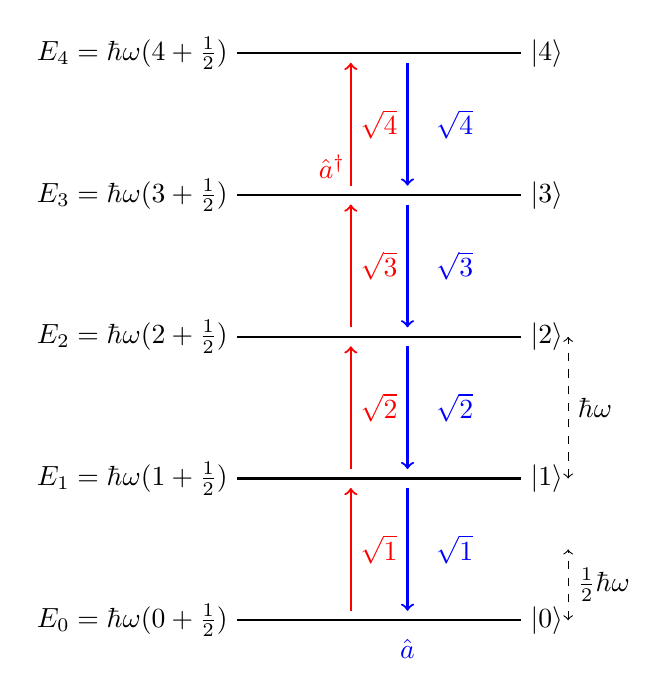
\begin{tikzpicture}[scale=1.2]
	% Niveles de energía
	\foreach \n in {0,1,2,3,4} {
		\draw[thick] (0,\n*1.5) -- (3,\n*1.5);
		\node[left] at (0,\n*1.5) {$E_{\n} = \hbar\omega(\n + \frac{1}{2})$};
		\node[right] at (3,\n*1.5) {$|{\n}\rangle$};
	}

	% Flechas de creación (rojas, hacia arriba)
\foreach \n in {0,1,2,3} {
	\pgfmathtruncatemacro{\m}{\n+1}
	\draw[->,red,thick] (1.2,\n*1.5+0.1) -- (1.2,\m*1.5-0.1);
	\node[red,right] at (1.2,\n*1.5+0.75) {$\sqrt{\m}$};
}
\node[red] at (1,4.8) {$\hat{a}^\dagger$};
		
		
		
		
		% Flechas de aniquilación (azules, hacia abajo)
	\foreach \n in {1,2,3,4} {
		\pgfmathtruncatemacro{\m}{\n-1}
		\draw[->,blue,thick] (1.8,\n*1.5-0.1) -- (1.8,\m*1.5+0.1);
		\node[blue,right] at (2,\n*1.5-0.75) {$\sqrt{\n}$};
	}
	\node[blue] at (1.8,-0.3) {$\hat{a}$};
	
	% Energía de punto cero
	\draw[<->,dashed] (3.5,0) -- (3.5,0.75);
	\node[right] at (3.5,0.375) {$\frac{1}{2}\hbar\omega$};
	\draw[<->,dashed] (3.5,1.5) -- (3.5,3);
	\node[right] at (3.5,2.25) {$\hbar\omega$};
	
\end{tikzpicture}

	\caption{Niveles de energía del oscilador armónico cuántico. Los operadores $\hat{a}^\dagger$ (rojo) y $\hat{a}$ (azul) actúan como escaleras, subiendo y bajando entre niveles con las constantes de normalización indicadas. El espaciado uniforme es $\hbar\omega$ y existe una energía de punto cero de $\frac{1}{2}\hbar\omega$. Fuente propia.}
	\label{fig:niveles}
\end{figure}




\subsection{Autofunciones del oscilador armónico en representación de posición}
\subsubsection{Autofunciones del oscilador armónico}

Los autoestados $|n\rangle$ obtenidos en la sección anterior son vectores abstractos en el espacio de Hilbert. Para calcular distribuciones de probabilidad y valores esperados de observables, necesitamos las \textbf{autofunciones} $\psi_n(x)$, que son las representaciones concretas de estos estados en el espacio de posición:

\begin{equation}
	\psi_n(x) = \langle x | n \rangle
\end{equation}

Las autofunciones son funciones de onda explícitas que podemos graficar y que satisfacen la ecuación de  \cite{schrodinger1926a} en forma de ecuación diferencial.

El resultado, derivado mediante el método analítico de \cite{schrodinger1926b} es:

\begin{equation}
	\psi_n(x) = \left(\frac{m\omega}{\pi\hbar}\right)^{1/4} \frac{1}{\sqrt{2^n n!}} H_n\left(\sqrt{\frac{m\omega}{\hbar}}x\right) \exp\left(-\frac{m\omega x^2}{2\hbar}\right)
	\label{eq:autofunciones}
\end{equation}

donde $H_n(\xi)$ son los polinomios de Hermite de orden $n$ (ver Apéndice~\ref{sec:hermite} para propiedades).


\subsubsection{Ortonormalidad}

Las autofunciones del oscilador armónico forman un conjunto \textbf{ortonormal}: son mutuamente ortogonales (perpendiculares en el sentido del producto interno) y cada una está normalizada (tiene norma unitaria). Matemáticamente:

\begin{equation}
	\int_{-\infty}^{\infty} \psi_n(x) \psi_m(x) dx = \delta_{nm}
\end{equation}

donde $\delta_{nm}$ es la delta de Kronecker:

\begin{equation}
	\delta_{nm} = \begin{cases} 
		1 & \text{si } n = m \\
		0 & \text{si } n \neq m
	\end{cases}
\end{equation}

\textbf{Ortogonalidad} ($n \neq m$): Funciones correspondientes a diferentes niveles de energía son mutuamente perpendiculares, reflejando que son estados físicamente distinguibles.

\textbf{Normalización} ($n = m$): Cada autofunción tiene probabilidad total igual a 1 de encontrar la partícula en algún lugar del espacio.


\subsubsection{Paridad}

Las funciones $\psi_n(x)$ tienen paridad bien definida:

\begin{equation}
	\psi_n(-x) = (-1)^n \psi_n(x)
\end{equation}

\textbf{Estados pares} ($n$ par): $\psi_n(-x) = +\psi_n(x)$ — función simétrica

\textbf{Estados impares} ($n$ impar): $\psi_n(-x) = -\psi_n(x)$ — función antisimétrica\\


\begin{figure}[h!]
	\centering
	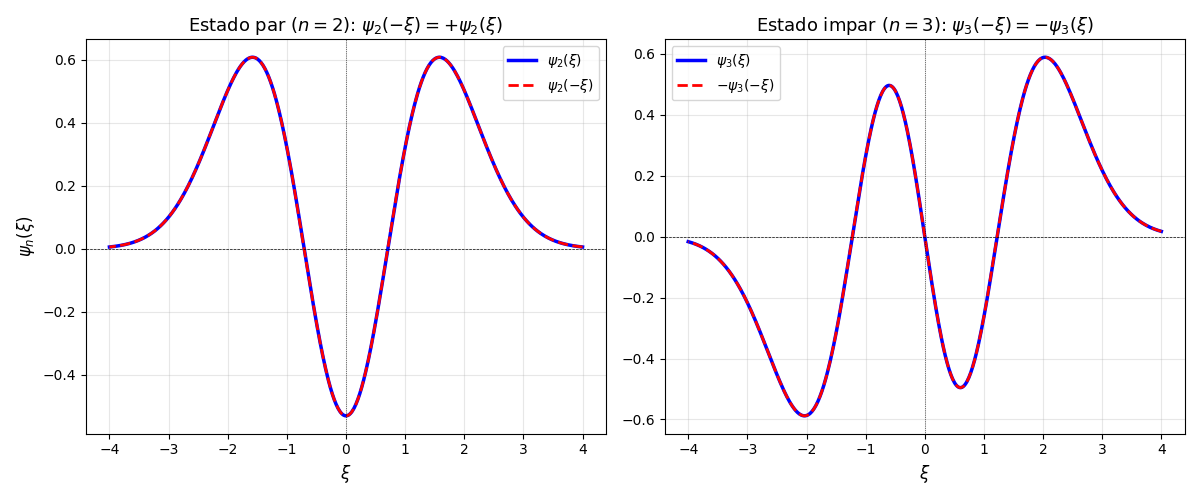
\includegraphics[width=1\linewidth]{paridad}
	\caption{Comparación paridad (estados pares vs impares). Fuente propia}
	\label{fig:paridad}
\end{figure}

\subsubsection{Número de nodos}

La función $\psi_n(x)$ tiene exactamente $n$ nodos (ceros):

\begin{itemize}
	\item $\psi_0(x)$: 0 nodos (gaussiana pura)
	\item $\psi_1(x)$: 1 nodo en $x = 0$
	\item $\psi_2(x)$: 2 nodos simétricos respecto al origen
	\item $\psi_n(x)$: $n$ nodos
\end{itemize}

Esta propiedad es general para problemas unidimensionales: el $n$-ésimo estado excitado tiene $n$ nodos.

\subsubsection{Funciones de onda de los primeros estados}

Usando la ecuación (\ref{eq:autofunciones}) y los primeros polinomios de Hermite (Apéndice ~\ref{sec:hermite}), obtenemos explícitamente:

\textbf{Estado fundamental ($n=0$):}
\begin{equation}
	\psi_0(x) = \left(\frac{m\omega}{\pi\hbar}\right)^{1/4} \exp\left(-\frac{m\omega x^2}{2\hbar}\right)
\end{equation}

Distribución gaussiana centrada en $x=0$ con ancho $\Delta x = \sqrt{\hbar/(2m\omega)}$.

\textbf{Primer estado excitado ($n=1$):}
\begin{equation}
	\psi_1(x) = \left(\frac{m\omega}{\pi\hbar}\right)^{1/4} \sqrt{\frac{2m\omega}{\hbar}} \, x \exp\left(-\frac{m\omega x^2}{2\hbar}\right)
\end{equation}

Función impar con un nodo en $x=0$.

\textbf{Segundo estado excitado ($n=2$):}
\begin{equation}
	\psi_2(x) = \left(\frac{m\omega}{\pi\hbar}\right)^{1/4} \frac{1}{\sqrt{2}}\left(\frac{2m\omega x^2}{\hbar} - 1\right) \exp\left(-\frac{m\omega x^2}{2\hbar}\right)
\end{equation}

Función par con dos nodos en $x = \pm\sqrt{\hbar/(2m\omega)}$.\\

\begin{table}[h]
	\centering
	\caption{Propiedades de los primeros estados del oscilador armónico cuántico}
	\label{tab:estados}
	\begin{tabular}{ccccl}
		\hline
		\textbf{Estado} & \textbf{Energía} & \textbf{Paridad} & \textbf{Nodos} & \textbf{Polinomio Hermite} \\
		$n$ & $E_n/(\hbar\omega)$ & Par/Impar & Cantidad & $H_n(\xi)$ \\
		\hline
		0 & 1/2 & Par & 0 & $1$ \\
		1 & 3/2 & Impar & 1 & $2\xi$ \\
		2 & 5/2 & Par & 2 & $4\xi^2 - 2$ \\
		3 & 7/2 & Impar & 3 & $8\xi^3 - 12\xi$ \\
		4 & 9/2 & Par & 4 & $16\xi^4 - 48\xi^2 + 12$ \\
		\hline
		\multicolumn{5}{l}{Patrón general: $E_n = \hbar\omega(n + \frac{1}{2})$, paridad = $(-1)^n$, nodos = $n$}
	\end{tabular}
\end{table}

	

\begin{figure}[H]
	\centering
	\includegraphics[width=0.8\linewidth]{"funciones de onda"}
	\caption{Ejemplos de funciones de onda $\psi_0, \psi_1, \psi_2, \psi_3$. Fuente propia}
	\label{fig:funciones-de-onda}
\end{figure}



\begin{figure}[H]
	\centering
	\includegraphics[width=0.8\linewidth]{"densidad de onda"}
	\caption{Ejemplos de densidades de probaiblidad $|\Psi_n|$ }
	\label{fig:densidad-de-onda}
\end{figure}



\subsection{Equivalencia entre el método analítico y el método algebraico}

Los métodos analítico y algebraico constituyen formulaciones matemáticamente equivalentes del mismo sistema físico. La identificación de esta equivalencia marcó uno de los hitos fundamentales en la consolidación de la mecánica cuántica, al demostrarse que la mecánica ondulatoria de Schrödinger y la mecánica matricial desarrollada por Heisenberg, Born y Jordan describen de manera consistente la misma estructura dinámica \citep{heisenberg1925, born1925, bornheisenberg1926, schrodinger1926a, schrodinger1926b}.


\subsubsection{Estado fundamental: comparación}

\textbf{Método analítico:} Para $n=0$, $H_0(\xi) = 1$, y la ecuación (\ref{eq:autofunciones}) da:

\begin{equation}
	\psi_0(x) = \left(\frac{m\omega}{\pi\hbar}\right)^{1/4} e^{-m\omega x^2/(2\hbar)}
\end{equation}

\textbf{Método algebraico:} La condición $\hat{a}|0\rangle = 0$ en representación de posición se traduce en:

\begin{equation}
	\sqrt{\frac{m\omega}{2\hbar}}\left(x + \frac{\hbar}{m\omega}\frac{d}{dx}\right)\psi_0(x) = 0
\end{equation}

Resolviendo esta ecuación diferencial ordinaria de primer orden:

\begin{equation}
	\frac{d\psi_0}{dx} = -\frac{m\omega}{\hbar} x \psi_0
\end{equation}

\begin{equation}
	\psi_0(x) = A e^{-m\omega x^2/(2\hbar)}
\end{equation}

Con normalización, $A = (m\omega/\pi\hbar)^{1/4}$.

\textbf{¡Ambos métodos dan la misma función!}

\subsubsection{Estados excitados: conexión}

En representación de posición, el operador $\hat{a}^\dagger$ actúa como \cite{dirac1930}:

\begin{equation}
	\hat{a}^\dagger \to \sqrt{\frac{m\omega}{2\hbar}}\left(x - \frac{\hbar}{m\omega}\frac{d}{dx}\right)
\end{equation}

Aplicando $(\hat{a}^\dagger)^n$ a $\psi_0(x)$ genera polinomios multiplicando la gaussiana, que son precisamente los polinomios de Hermite multiplicados por la constante apropiada \citep{sakurai2020}.

\subsubsection{Interpretación física}

\textbf{Método analítico \citep{schrodinger1926b}} :
\begin{itemize}
	\item Proporciona funciones de onda explícitas en representación de posición
	\item Visualización directa de densidades de probabilidad $|\psi_n(x)|^2$
	\item Útil para cálculos de valores esperados de observables
	\item Permite entender el comportamiento espacial de estados cuánticos
\end{itemize}

\textbf{Método algebraico \citep{dirac1930}} :
\begin{itemize}
	\item Más elegante y general
	\item No requiere resolver ecuaciones diferenciales
	\item Se generaliza fácilmente a otros sistemas
	\item Lenguaje natural para describir excitaciones (fonones, fotones) en sistemas de muchos cuerpos
	\item Lenguaje natural para describir excitaciones (fonones, fotones) en sistemas de muchos cuerpos y en teorías cuánticas de campos

\end{itemize}

\begin{table}[h]
	\centering
	\caption{Comparación entre el método analítico (Schrödinger) y algebraico (Dirac)}
	\label{tab:comparacion_metodos}
	\begin{tabular}{p{4cm}p{5cm}p{5cm}}
		\hline
		\textbf{Aspecto} & \textbf{Método analítico} & \textbf{Método algebraico} \\
		\hline
		Formulación & Ecuación diferencial & Álgebra de operadores \\
		Herramienta principal & Polinomios de Hermite & Operadores escalera $\hat{a}$, $\hat{a}^\dagger$ \\
		Resultado directo & Autofunciones $\psi_n(x)$ & Espectro $E_n$ y autoestados $|n\rangle$ \\
		Complejidad matemática & Alta (EDOs, series) & Media (álgebra) \\
		Visualización & Directa ($|\psi_n(x)|^2$) & Requiere proyección \\
		Generalización & Específica al OAC & Se generaliza fácilmente \\
		\hline
	\end{tabular}
\end{table}


A lo largo de esta sección hemos derivado completamente el espectro de energía $E_n = \hbar\omega(n + \frac{1}{2})$ y las autofunciones $\psi_n(x)$ del oscilador armónico cuántico mediante el método desarrollado por \cite{dirac1930} y entendimos las equivalencias con el método desarrollado por \cite{schrodinger1926b}. La equivalencia matemática de ambos enfoques confirma la consistencia interna de la mecánica cuántica y demuestra que diferentes formalismos pueden describir el mismo sistema físico. Esta dualidad ha sido fundamental en el desarrollo de la física cuántica moderna, desde la teoría cuántica de campos hasta las aplicaciones contemporáneas en computación cuántica.





\section{Aplicaciones físicas del oscilador armónico cuántico}
\subsection{Vibraciones atómicas y moleculares}

\subsection{Fonones y vibraciones colectivas en sólidos}

\subsection{Osciladores cuánticos como modos bosónicos fundamentales}